\documentclass[11pt]{article}
\usepackage{enumerate}
\usepackage{fullpage}
\usepackage{fancyhdr}
\usepackage{amsmath, amsfonts, amsthm, amssymb}
\usepackage{mathrsfs}
\usepackage{graphicx}
\setlength{\parindent}{0pt}
\setlength{\parskip}{5pt plus 1pt}
\pagestyle{empty}

\def\indented#1{\list{}{}\item[]}
\let\indented=\endlist

\newcounter{questionCounter}
\newcounter{partCounter}[questionCounter]
\newenvironment{question}[2][\arabic{questionCounter}]{%
    \setcounter{partCounter}{0}%
    \vspace{.25in} \hrule \vspace{0.5em}%
        \noindent{\bf #2}%
    \vspace{0.8em} \hrule \vspace{.10in}%
    \addtocounter{questionCounter}{1}%
}{}
\renewenvironment{part}[1][\alph{partCounter}]{%
    \addtocounter{partCounter}{1}%
    \vspace{.10in}%
    \begin{indented}%
       {\bf (#1)} %
}{\end{indented}}

%%%%%%%%%%%%%%%%%%%%%%%HEADER%%%%%%%%%%%%%%%%%%%%%%%%%%%%%%
\newcommand{\myname}{Shashank Singh\footnote{sss1@andrew.cmu.edu}}
\newcommand{\myclass}{21-470 Calculus of Variations}
\newcommand{\myhwnum}{3}
\newcommand{\duedate}{Friday, February 14, 2014}
%%%%%%%%%%%%%%%%%%%%%%%%%%%%%%%%%%%%%%%%%%%%%%%%%%%%%%%%%%%

%%%%%%%%%%%%%%%%%%%%CONTENT MACROS%%%%%%%%%%%%%%%%%%%%%%%%%
\renewcommand{\qed}{\quad \ensuremath{\blacksquare}}
\newcommand{\inv}{^{-1}}
\newcommand{\bv}{\mathbf{v}}
\newcommand{\bx}{\mathbf{x}}
\newcommand{\by}{\mathbf{y}}
\newcommand{\bff}{\mathbf{f}}
\newcommand{\bzero}{\mathbf{0}}
\newcommand{\bxi}{\boldsymbol{\xi}}
\newcommand{\boldeta}{\boldsymbol{\eta}}
\newcommand{\dist}{\operatorname{dist}} % distance from or between sets
\newcommand{\area}{\operatorname{area}} % area of a polygon
\newcommand{\Gr}{\operatorname{Gr}}     % graph of a function
\renewcommand{\sp}{\operatorname{span}} % span of a set
\newcommand{\bdry}{\operatorname{bdry}} % boundary of a set
\newcommand{\sminus}{\backslash}        % set difference
\newcommand{\N}{\mathbb{N}}             % natural numbers
\newcommand{\Z}{\mathbb{Z}}             % integers
\newcommand{\Q}{\mathbb{Q}}             % rational numbers
\newcommand{\R}{\mathbb{R}}             % real numbers
\newcommand{\C}{\mathbb{C}}             % complex numbers
\newcommand{\D}{\mathcal{D}}            % domain of an operator
\newcommand{\Cmp}{\mathcal{C}}          % space of compact linear operators\s
\newcommand{\K}{\mathbb{K}}             % underlying field of a linear space
\newcommand{\Ran}{\mathcal{R}}          % range of a linear operator
\newcommand{\Nul}{\mathcal{N}}          % null-space of a linear operator
\renewcommand{\L}{\mathcal{L}}          % space of bounded linear functions
\newcommand{\pow}[1]{\mathcal{P}\left(#1\right)}    % power set of #1
\newcommand{\e}{\varepsilon}            % \varepsilon
\newcommand{\wto}{\rightharpoonup}      % weak convergence
\newcommand{\wsto}{\stackrel{*}{\rightharpoonup}}   % weak-* convergence
\renewcommand{\Re}{\operatorname{Re}}   % real part of a complex number
\newcommand{\tT}{\widetilde{T}}         % for P3
\newcommand{\A}{\mathcal{A}}            % for P3
\renewcommand{\S}{\mathcal{S}}          % Schwartz space
\newcommand{\X}{\mathscr{X}}            % entire linear space
\newcommand{\Y}{\mathscr{Y}}            % domain of objective functional
\newcommand{\V}{\mathscr{V}}            % set of admissible variations
%%%%%%%%%%%%%%%%%%%%%%%%%%%%%%%%%%%%%%%%%%%%%%%%%%%%%%%%%%%

\begin{document}
\thispagestyle{plain}

{\Large Homework \myhwnum} \\
\myclass \\
Name: \myname \\
Due: \duedate

\begin{question}{Problem 1}
Figure \ref{fig:Bbeta} and Table \ref{tab:Bbeta} show the relationship between
$\beta$ and $B$.
\vspace{-3mm}
\begin{figure}[h]
\begin{center}
\includegraphics[width=0.65\textwidth]{B_over_beta}
\end{center}
\vspace{-9mm}
\caption{Plot of $B$ over $\beta \in (-1,0.6)$. $B$
values selected in Table \ref{tab:Bbeta} are marked by dotted lines.}
\label{fig:Bbeta}
\end{figure}
\vspace{-5mm}
\begin{table}[h]
\centering
\begin{tabular}{c*{5}{|c}}
B       &   0       &   0.1     &   1       &   2       &   4   \\
\hline
$\beta$ &   -0.5471 &   -0.4178 &   0.3649  &   0.5454  &   0.5841
\end{tabular}
\caption{Values of $\beta$ for selected values of $B$}
\label{tab:Bbeta}
\end{table}
\vspace{-2mm}

Observing that $B$ increases monotonically with $\beta$, the $\beta$
corresponding to each $B$ was computed numerically using the following
iterative procedure:
\vspace{-3mm}
\begin{verbatim}
beta_H <- 0.586; beta_L <- -0.8
while beta_H - beta_L > 0.0001
  beta_A <- (beta_H + beta_L)/2
  if B(beta_A) > B
    beta_H <- beta_A
  else
    beta_L <- beta_A
return beta_L
\end{verbatim}
\vspace{-2mm}
where $B(\beta_A)$ was computed by numerically integrating Equation (6).
\end{question}

\begin{question}{Problem 2}
\begin{figure}[h]
\begin{center}
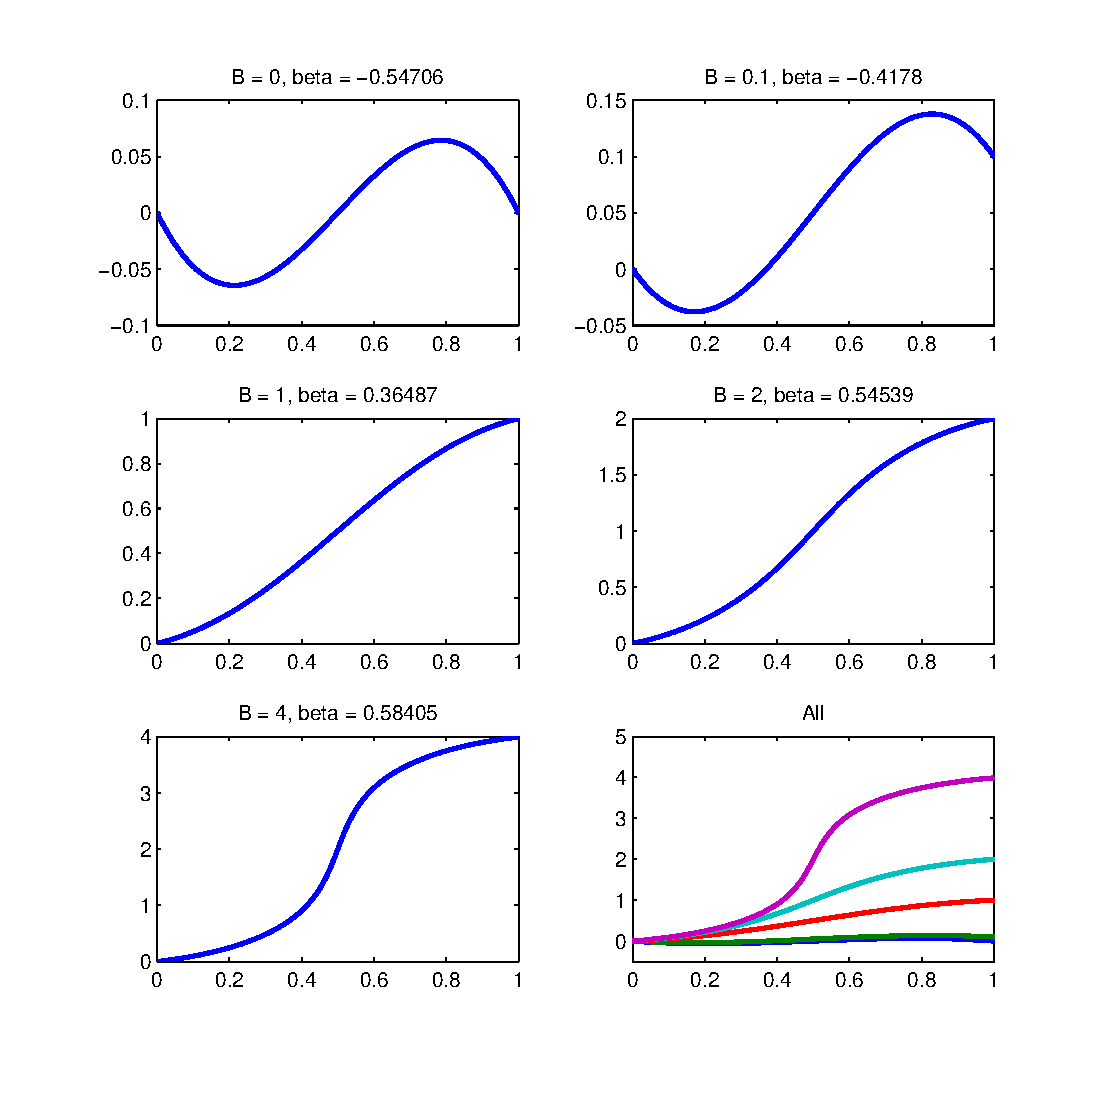
\includegraphics[width=0.8\textwidth]{ygraphs}
\end{center}
\vspace{-9mm}
\caption{Graphs of $y$ for $B = 0,0.1,1,2,4$, computed from
equation (6) and $\beta$ values in Table \ref{tab:Bbeta}. The last plot shows
all 5 graphs, for comparison.}
\label{fig:ygraphs}
\end{figure}
\end{question}

\newpage
\begin{question}{Problem 3}
Figure \ref{fig:Bbeta} suggests that $\beta$ is roughly a sigmoid function of
$B$. A least squares approximation to a sample of $\beta$ points gives
\[\beta(B) \approx \frac{0.56+1.3}{1+10^{1.1(0.12-B)}}-1.3,\]
as illustrated in Figure \ref{fig:betaB}.
\begin{figure}[h]
\begin{center}
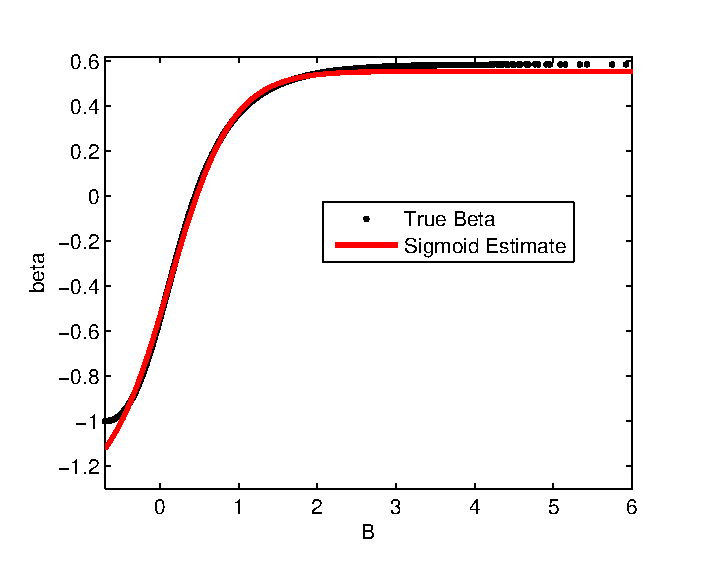
\includegraphics[width=0.65\textwidth]{betaB}
\end{center}
\vspace{-9mm}
\caption{Plot of $\beta$ over $B$ and a fitted sigmoid function.}
\label{fig:betaB}
\end{figure}
The case $\beta \geq 0$ results in a path ($y$) that is
monotonically increasing in time and $x$, whereas, when $\beta < 0$, the path
is more sinusoidal, and, $y$ is not monotonically increasing. This corresponds
roughly to $B = 0.45$.
\end{question}
\end{document}
